\documentclass{article}

% Recommended, but optional, packages for figures and better typesetting:
\usepackage{microtype}
\usepackage{graphicx}
\usepackage{subfigure}
\usepackage{booktabs} 
\usepackage[utf8]{inputenc} 
\usepackage{hyperref}
\usepackage{caption}
\usepackage{amssymb}

% Attempt to make hyperref and algorithmic work together better:
\newcommand{\theHalgorithm}{\arabic{algorithm}}

% Use the following line for the initial blind version submitted for review:
\usepackage[accepted]{icml2021}

\icmltitlerunning{Multimodal Emotion Recognition}

\begin{document}


\twocolumn[
\icmltitle{Multimodal Emotion Recognition}
\icmlsetsymbol{equal}{*}

\begin{icmlauthorlist}
\icmlauthor{Shuang Cai}{equal,aff1}
\icmlauthor{Rongchuan Zhang}{equal,aff2}
\icmlauthor{Mahdi Jafarkhani}{equal,aff2}
\end{icmlauthorlist}

\icmlaffiliation{aff1}{Department of Computational Linguistics, University of Stuttgart, Stuttgart, Germany}
\icmlaffiliation{aff2}{Department of Computer Science, University of Stuttgart, Stuttgart, Germany}

\vskip 0.3in
]

% this must go after the closing bracket ] following \twocolumn[ ...

% This command actually creates the footnote in the first column
% listing the affiliations and the copyright notice.
% The command takes one argument, which is text to display at the start of the footnote.
% The \icmlEqualContribution command is standard text for equal contribution.
% Remove it (just {}) if you do not need this facility.

\printAffiliationsAndNotice{}  % leave blank if no need to mention equal contribution

\begin{abstract}
Multimodal Emotion Recognition (MER) plays a vital role in understanding human emotions by integrating data from text, audio, and video modalities. This study evaluates the performance of various architectures, including Early Fusion, Late Fusion, Multimodal Factorization Models (MFM), Multimodal Transformers (MulT), and Multimodal Cyclic Translation Networks (MCTN), on two benchmark datasets: CMU-MOSI and CMU-MOSEI. Additionally, Unimodal baselines are incorporated for comparison to assess the added value of multimodal integration. By analyzing model performance across datasets, we identify the unique challenges and strengths of each architecture, providing insights into their suitability for diverse multimodal contexts. This work offers valuable guidance for advancing sentiment analysis through effective multimodal architectures. Our code and experiment results are available on the \href{https://github.com/M-Jafarkhani/Multimodal-Emotion-Recognition}{GitHub}.
\end{abstract}

\section{Introduction}
Emotion recognition is a crucial subfield of affective computing, aiming to identify and analyze human emotions expressed across different modalities, such as text, audio, and video. While traditional emotion recognition methods focused on single modalities like text, recent advancements in multimodal analysis provide deeper insights into how humans express emotions in diverse contexts. Multimodal Emotion Recognition (MER) integrates signals from multiple data sources, addressing the limitations of unimodal approaches and capturing the intricate relationships between modalities.

In this study, we aim to explore the effectiveness of various emotion recognition models across two prominent datasets: CMU-MOSI and CMU-MOSEI. Our work evaluates the performance of different models and fusion techniques on these datasets. By focusing on these differences, this paper provides insights into the impact of dataset structure and context on multimodal emotion recognition. The findings contribute to advancing MER methodologies and understanding the specific challenges posed by multi-modalities tracking.

\section{Article Review}
\subsection{Overview of Emotion Recognition in Multi-modal Data}
Recent studies have highlighted the effectiveness of deep neural networks in capturing the complexity of emotional expressions in multiple modalities. The CMU-MOSEI\cite{bagher-zadeh-etal-2018-multimodal} and CMU-MOSI\cite{Zadeh2016MOSIMC} multimodal datasets are widely used benchmarks to address emotion recognition tasks.

\textbf{CMU-MOSI} (CMU Multimodal Opinion Sentiment Intensity) is a dataset introduced by Carnegie Mellon University (CMU) that focuses on extracting and analyzing sentiment polarity from multimodal data. It is one of the earliest datasets widely used for multi-modal sentiment analysis. The dataset comprises 93 videos with a total of 2,199 segments, incorporating three modalities: text, visual, and audio. Specifically, it targets sentiment intensity, with annotations on a polarity scale ranging from [-3, 3]. CMU-MOSI is well suited for tasks involving multimodal sentiment intensity analysis, exploring emotional expression in monologue settings, and studying cross-modal feature interactions.

\textbf{CMU-MOSEI} (CMU Multimodal Opinion Sentiment and Emotion Intensity) is an extended version of CMU-MOSI, offering a larger and more diverse corpus for multi-modal sentiment analysis. It includes 23,453 video segments from more than 1,000 speakers, covering more than 250 topics. Similar to CMU-MOSI, it features text, visual, and audio modalities. In addition to sentiment polarity scores, it provides annotations for six emotions: happiness, sadness, anger, fear, disgust, and surprise. This multi-label characteristic shows the complexity of human expression and allows models to learn a richer representation of emotional content.

\subsection{Overview of Multi-modal Model on Emotion Recognition Task}
Multi-modal models for emotion recognition tasks have attracted significant attention in recent years. A key challenge in multi-modal learning lies in effectively fusing different types of data into a unified representation that can be utilized for training, enabling the model to extract comprehensive multi-modal features and enhance its performance. Among the commonly employed feature fusion techniques, Early Fusion and Late Fusion are early and widely used \cite{Baltruaitis2017MultimodalML}. Early Fusion involves combining input features from different modalities (e.g., text, audio, video) into a unified multi-modal representation before being processed by the model. This unified representation is then fed into a GRU for further processing. In contrast, Late Fusion integrates the outputs from independently modeled modalities. Each modality is processed separately by an independent model to generate individual representations or predictions, which are subsequently combined through methods such as averaging, weighting, or classifier-based fusion to achieve the final output.

Early Fusion is conceptually simpler and leverages inter-modal relationships effectively. However, it may compromise the independence of individual modalities. On the other hand, Late Fusion ensures stronger independence of modalities, making it easier to fine-tune each component. Nonetheless, it has weaker inter-modal interactions since the fusion occurs at the final stage. (Figure \ref{fig:early-late-fusion})

\begin{figure}[ht]
    \centering
    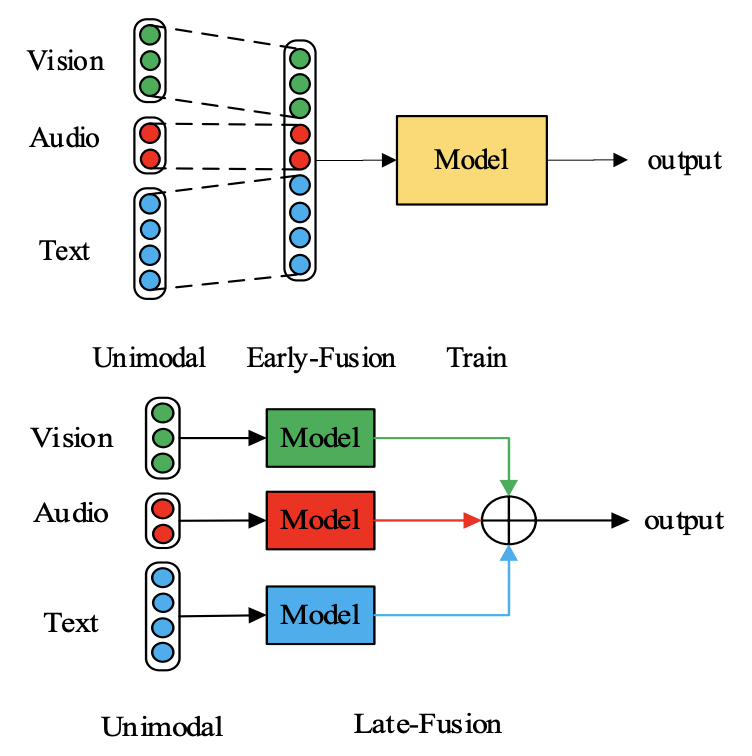
\includegraphics[width=1\linewidth]{Foundation model draft1//figs/Early and Late Fusion.png}
    \caption{Early (upper) and Late Fusion (lower) \cite{Wu2022}}
    \label{fig:early-late-fusion}
\end{figure}

With the emergence of the Transformers, researchers naturally began applying them to Early Fusion methods due to their ability to effectively capture global dependencies among input features. MulT \cite{tsai-etal-2019-multimodal} is among the first works to introduce Transformers into multi-modal learning, leveraging a cross-modal self-attention mechanism to jointly model aligned or unaligned sequences from multiple modalities. Late Fusion methods based on Transformers typically involve independent modeling of each modality's input using separate Transformer encoders. The outputs from these encoders are then fused for the final task. For example, VideoBERT \cite{Sun2019VideoBERT} employs separate Transformer models to encode video frame sequences and language sequences independently, followed by a task-specific head module to integrate the outputs from both modalities for fusion and prediction. (Figure \ref{fig:mult-1})

\begin{figure}[h]
    \centering
    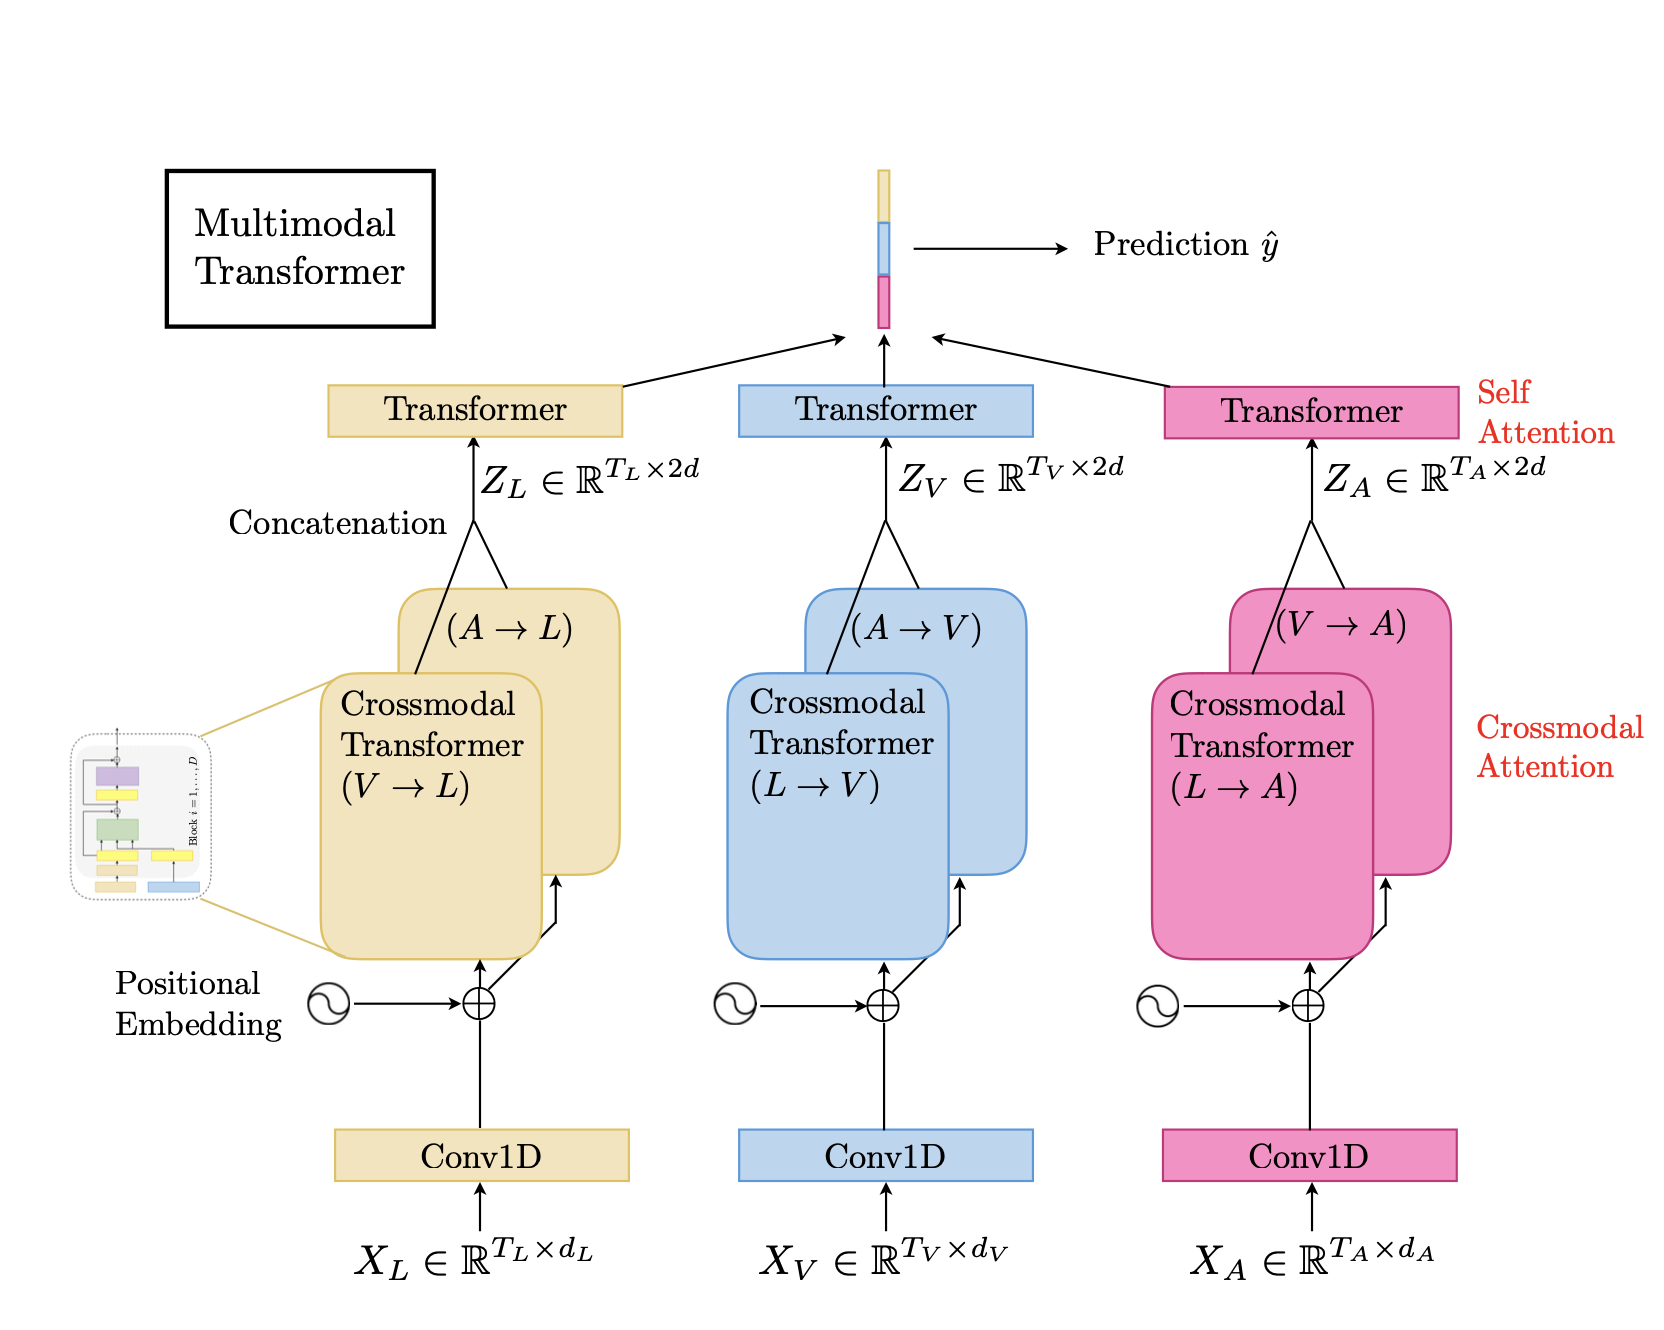
\includegraphics[width=1\linewidth]{Foundation model draft1//figs/Mult-1.png}
    \caption{Overall architecture for MulT on modalities $(L,V,A)$. The crossmodal transformers, which suggests latent crossmodal adaptations, are the core components of MulT for multimodal fusion. \cite{tsai-etal-2019-multimodal}}
    \label{fig:mult-1}
\end{figure}

Tensor Fusion \cite{zadeh-etal-2017-tensor} is an advanced fusion technique used in multi-modal learning, which constructs high-order tensors to capture interactions between different modalities. Unlike simple feature concatenation, Tensor Fusion preserves more complex high-order interaction information across modalities. However, this approach can result in high-dimensional tensors that may contain excessive, redundant information, increasing the risk of model overfitting. To address this issue, Low-Rank Tensor Fusion (LRTF) \cite{Liu2018EfficientLM} projects modality features into a low-rank space, reducing the tensor's dimensionality and thereby mitigating computational complexity and over-fitting risks. (Figure \ref{fig:tensor-fusion})

\begin{figure}[h]
    \centering
    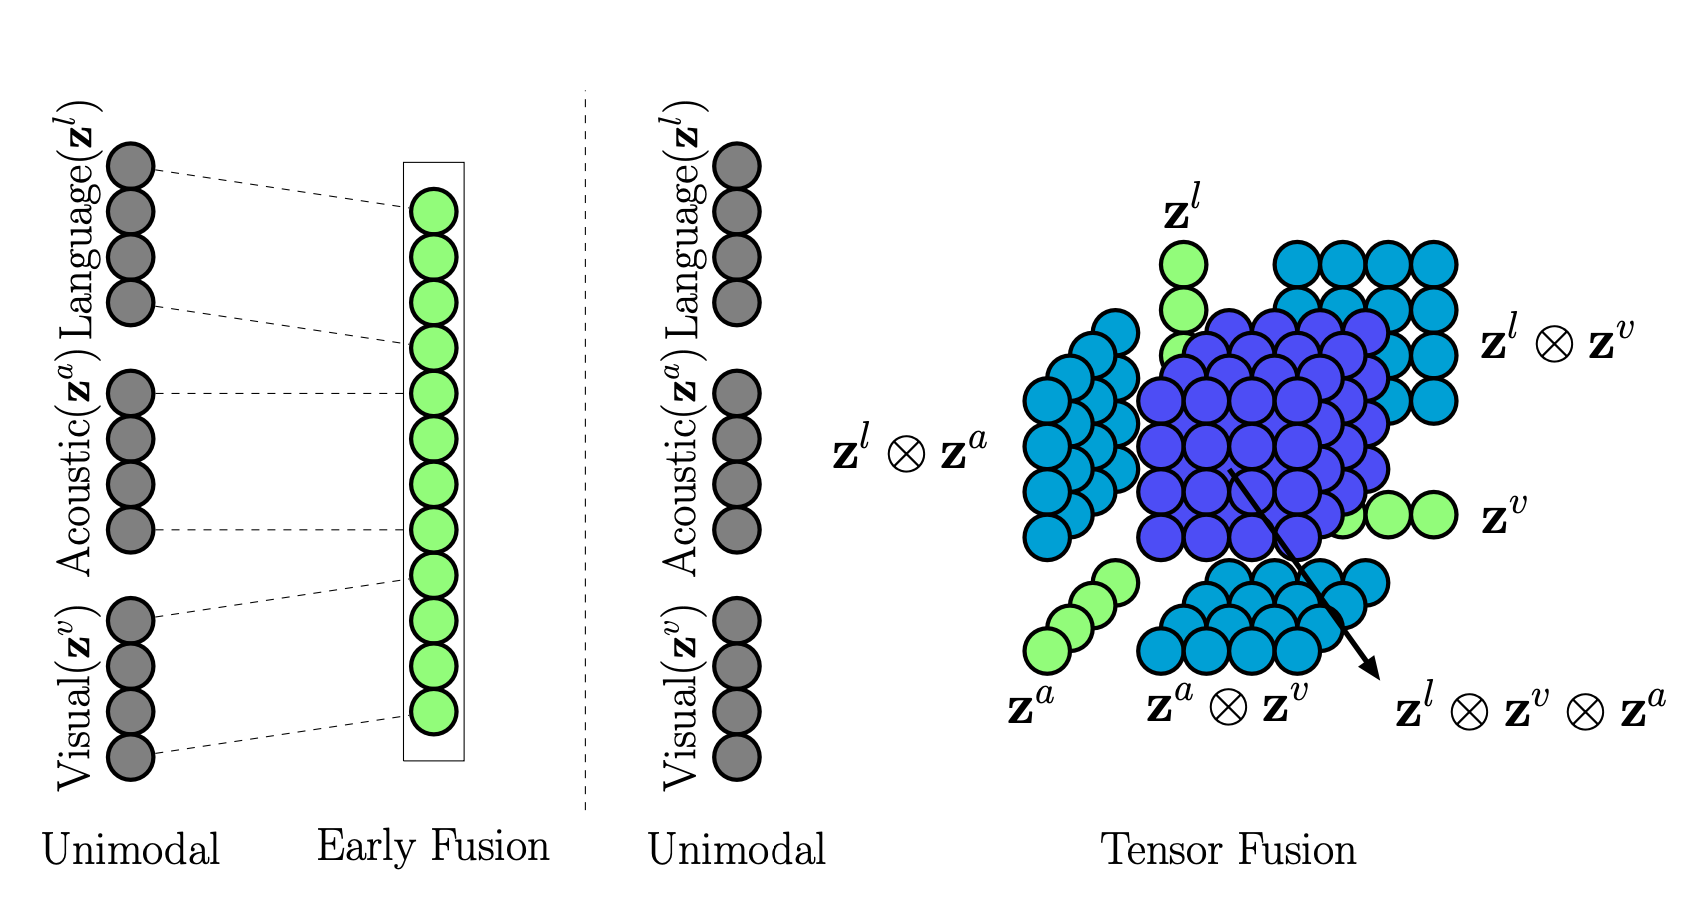
\includegraphics[width=1\linewidth]{Foundation model draft1//figs/tensor fusion.png}
    \caption{Commonly used early fusion (multimodal concatenation). Right: Tensor fusion with three types of subtensors: unimodal, bimodal, and trimodal. \cite{zadeh-etal-2017-tensor}}
    \label{fig:tensor-fusion}
\end{figure}

Joint Learning of Modalities is another popular fusion technique that focuses on modeling interactions between modalities or leveraging shared representations to enable collaborative learning across multi-modal data. This approach typically employs joint optimization objectives and carefully designed architectures to enhance inter-modal collaboration. One such approach is the Multi-modal Factorized Model (MFM) \cite{FactorizedMult}, which uses modality-specific encoders to generate latent representations while reconstructing the original data from a shared representation through decoders. This ensures that the shared representation retains sufficient modality-specific information. (Figure \ref{fig:factorized})

\begin{figure}[h]
    \centering
    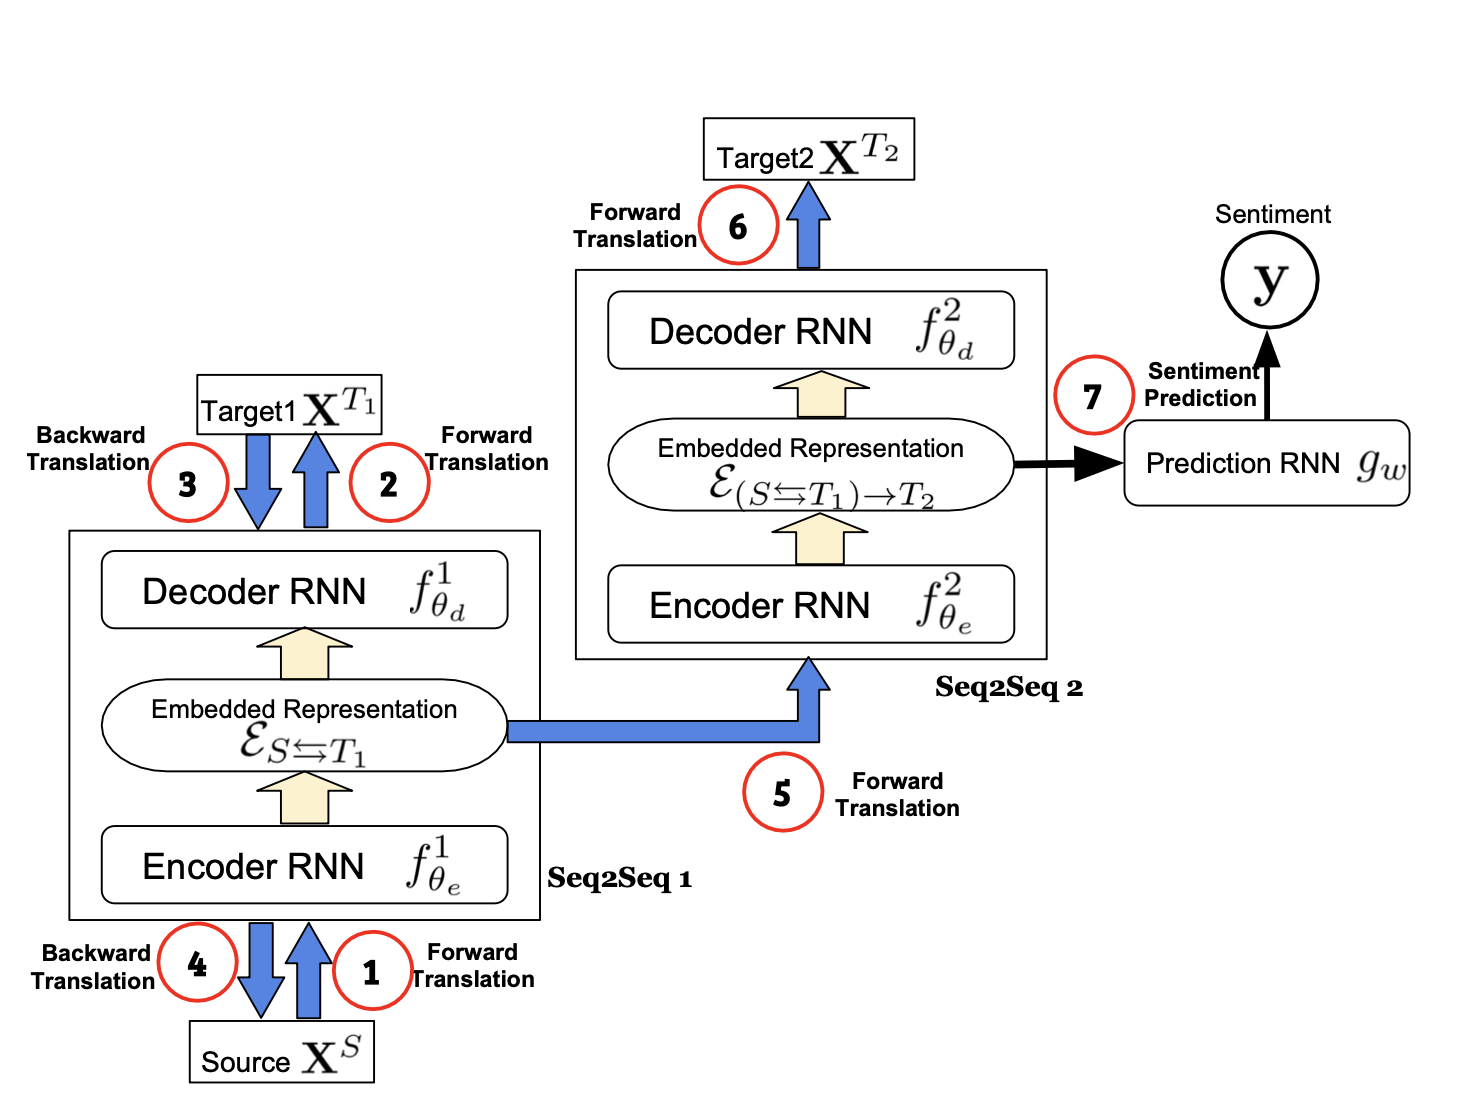
\includegraphics[width=1\linewidth]{Foundation model draft1//figs/MCTN.png}
    \caption{Hierarchical MCTN for three modalities: the source modality $\mathbf{X}^S$ and the target modalities $\mathbf{X}^{T_1}$ and $\mathbf{X}^{T_2}$. The joint representation $\mathcal{E}_{S \rightleftarrows T_1}$ is obtained via a cyclic translation between $\mathbf{X}^S$ and $\mathbf{X}^{T_1}$, then further translated into $\mathbf{X}^{T_2}$. Next, the joint representation of all three modalities, $\mathcal{E}_{(S \rightleftarrows T_1) \rightarrow T_2}$, is used for sentiment prediction. The model is trained end-to-end with a coupled translation-prediction objective. At test time, only the source modality $\mathbf{X}^S$ is required for prediction. \cite{Pham2019MCTN} }
    \label{fig:MCTN}
\end{figure}

\begin{figure*}[h]
    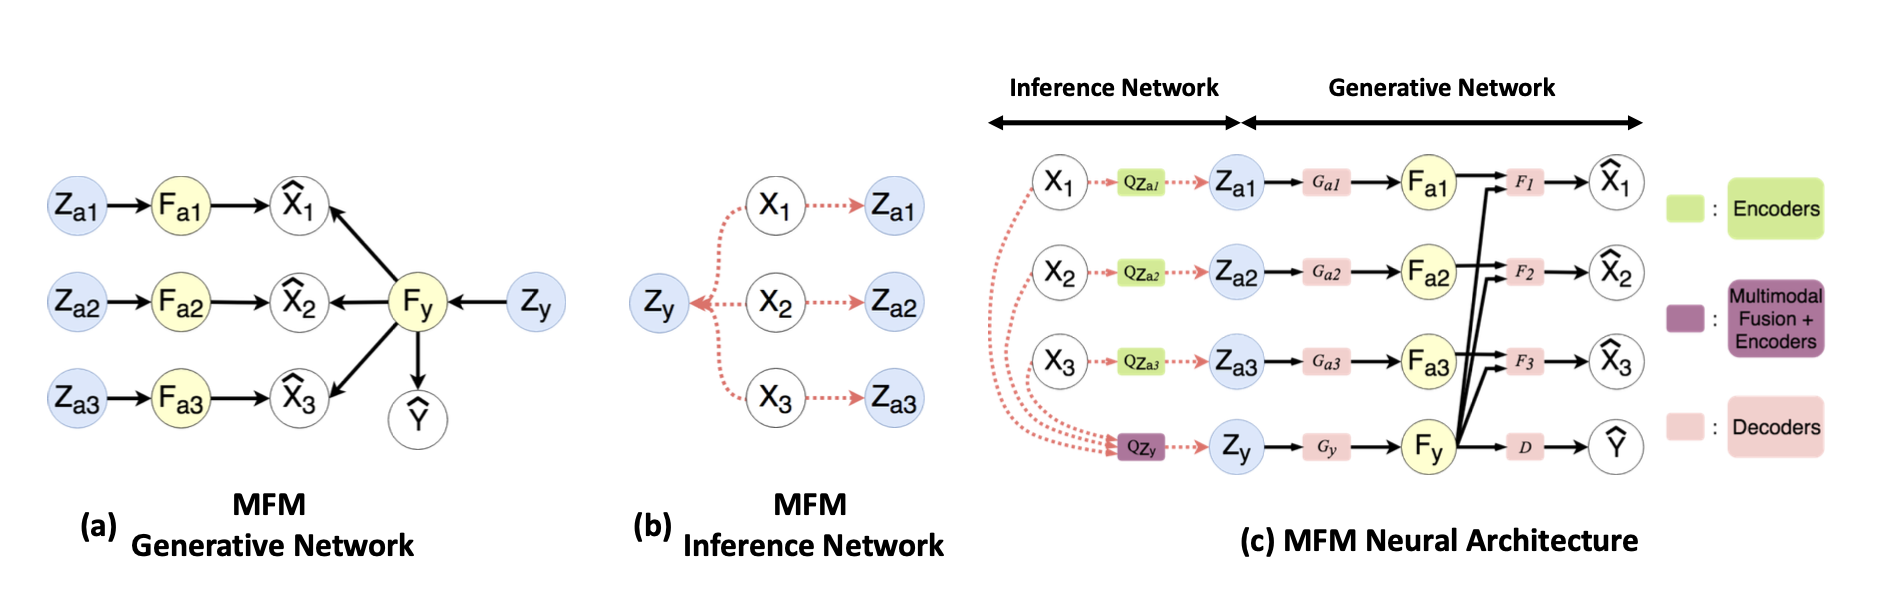
\includegraphics[width=1\linewidth]{Foundation model draft1//figs/Factorized.png}
\caption{Illustration of the Multimodal Factorization Model (MFM) with three modalities. MFM factorizes multimodal representations into \textit{multimodal discriminative} factors $\mathbf{F}_y$ and \textit{modality-specific generative} factors $\mathbf{F}_{a\{1:M\}}$. (a) MFM Generative Network with latent variables $\{\mathbf{Z}_y, \mathbf{Z}_{a\{1:M\}}\}$, factors $\{\mathbf{F}_y, \mathbf{F}_{a\{1:M\}}\}$, generated multimodal data $\hat{\mathbf{X}}_{1:3}$ and labels $\hat{\mathbf{Y}}$. (b) MFM Inference Network. (c) MFM Neural Architecture. Best viewed zoomed in and in color. \cite{FactorizedMult}}
    \label{fig:factorized}
\end{figure*}

Another example is the Multi-modal Cyclic Translation Network (MCTN) \cite{Pham2019MCTN}, which employs cyclic translation learning to achieve joint learning by iteratively training encoders and decoders to facilitate effective modality integration. (Figure \ref{fig:MCTN})


\section{Approaches}

\subsection{Experiment Setup}
We evaluate the foundation models for multimodal emotion recognition across two key datasets: \textbf{CMU-MOSI} and \textbf{CMU-MOSEI}. The experimental setup emphasizes meticulous pre-processing, robust feature extraction, and effective fusion of text, audio, and visual modalities to maximize model performance. The key components are as follows:

\begin{itemize} 
\item \textbf{Data Preprocessing and Feature Extraction:}
All datasets are first synchronized and aligned using the P2FA forced aligner to ensure temporal consistency across modalities. For the textual modality, video segment transcripts are converted into 300-dimensional vectors using pre-trained GloVe embeddings. For the visual modality, facial features—including facial action units and landmarks—are extracted with the Facet library and the OpenFace tool to generate sequences that capture facial expressions over time. For the audio modality, features are derived using the COVAREP toolkit, which extracts tone variations through 12 Mel-frequency cepstral coefficients along with additional relevant parameters.

    \item \textbf{Fusion Techniques:} We explore Early Fusion, Late Fusion and advanced approaches like Tensor Fusion, Low-Rank Tensor Fusion (LRTF), Multimodal Cyclic Translation Networks (MCTN) and Multimodal Transformers (MulT). These methods facilitate integration across modalities to harness cross-modal correlations effectively.
    \item \textbf{Model Architectures:} The experiments implement both traditional architectures (e.g., GRUs for sequence modeling) and transformer-based models for handling temporal and cross-modal dependencies.
    \item \textbf{Optimization and Training:} We use the Adam optimizer with a learning rate of \(10^{-4}\), weight decay of \(10^{-2}\), and early stopping based on validation metrics. Loss functions include cross-entropy for classification and L1/L2 loss for regression tasks.
\end{itemize}

\subsection{Experiment Result on Different Models}

Table~\ref{model-performance} represents the performance of various architectures across the datasets, highlighting the strengths and weaknesses of each approach.

\subsection{Findings}

\begin{itemize}
    \item \textbf{Fusion Strategies:} Early Fusion (Transformer) consistently achieves higher performance on CMU-MOSI and CMU-MOSEI datasets due to its ability to capture long-term dependencies in sequences.\\
    Late Fusion (Transformer) delivers competitive results while offering better modularity and interpretability.\\

    \item \textbf{Transformer Models:} 
    The Multimodal Transformer (MulT) shows strong performance across datasets, particularly on CMU-MOSEI, with an accuracy of 71.91\%. Its cross-modal attention mechanism enables effective interaction modeling between modalities.\\
    
    \item \textbf{Advanced Fusion Techniques:} 
    Tensor Fusion and its low-rank variant achieve solid results but are computationally expensive and prone to overfitting, as seen in the slightly lower performance of LRTF.\\
    
    \item \textbf{Error Analysis:}
    Misclassifications often occur in overlapping emotional categories (e.g., "neutral" and "sadness") and noisy modalities (e.g., inconsistent visual features). Future work should address these limitations through data augmentation and attention-based refinement.
\end{itemize}

\begin{table*}[h]
\centering
\resizebox{\linewidth}{!}{
\begin{tabular}{lccc}
\toprule
\textbf{Architecture} & \textbf{CMU-MOSI Accuracy (\%)} & \textbf{CMU-MOSEI Accuracy (\%)} & \textbf{Parameters (Million)} \\
\midrule
Early Fusion (Transformer) & \textbf{75.65} & \textbf{71.91} & $\sim$8.1 \\
Late Fusion (GRU) & 75.21 & 71.60 & $\sim$2.5 \\
Multimodal Transformer & 75.21 & 70.40 & $\sim$3.0 \\
Late Fusion (Transformer) & 73.32 & 68.49 & $\sim$20.0 \\
Multimodal Cyclic Translation Network & 72.44 & 59.49 & $\sim$0.2 \\
Tensor Fusion & 72.30 & 70.45 & $\sim$5.4 \\
Low Rank Tensor Fusion & 72.01 & 70.95 & $\sim$1.5 \\
%Unimodal & 71.28 & 70.01 & $\sim$1.9 \\
Early Fusion (GRU) & 66.90 & 49.01 & $\sim$1.6 \\
Multimodal Factorization & 63.70 & 56.88 & $\sim$1.4 \\
\bottomrule
\end{tabular}
}
\captionsetup{margin=10pt,font=small,labelfont=bf}
\caption{Performance of various architectures across datasets.}
\label{model-performance}
\end{table*}

\section{Analysis}

\subsection{Model Performance Comparison}
In our experiments on Early Fusion and Late Fusion, we employed GRU and Transformer as encoders, respectively. GRU (Gated Recurrent Unit) is a variant of the Recurrent Neural Network (RNN), designed to address the vanishing gradient problem in long-sequence processing. By introducing a gating mechanism, GRU selectively retains relevant information while discarding less useful details, making it effective for unimodal time-series modeling. However, its ability to handle high-dimensional and multimodal data is limited, as it lacks explicit mechanisms for capturing inter-modal interactions. In contrast, Transformers eliminates the recurrence structure entirely and instead leverages self-attention mechanisms to model sequential data, significantly enhancing its expressive power. The self-attention mechanism enables deep interactions across modalities, making it particularly suitable for multimodal fusion tasks. This explains why early fusion models perform exceptionally well with Transformer-based encoders in our experiments. Since Early Fusion integrates multiple modalities at an early stage before feeding them into the encoder, using a Transformer allows the model to effectively process the fused multimodal data. Conversely, in Late Fusion, each modality is first processed separately by the encoder and only merged at the final classification stage. In this case, GRU serves as a more effective encoder because it specializes in handling sequential information for individual modalities before fusion.


Tensor Fusion (TF) is a multimodal fusion technique designed to capture high-order interactions among text (T), audio (A), and visual (V) modalities. Unlike traditional Early Fusion, which simply concatenates features, Tensor Fusion computes the outer product of all modalities, resulting in a high-dimensional tensor representation that encapsulates complex inter-modal interactions. However, Tensor Fusion suffers from an exponential increase in computational cost. To mitigate this, Low-Rank Tensor Fusion (LRTF) \cite{Liu2018EfficientLM} was introduced as an optimized variant (Figure \ref{fig:LRTF}). LRTF applies low-rank decomposition to approximate the high-dimensional tensor with multiple lower-dimensional matrices, thereby significantly reducing the computational burden while preserving critical modal interactions. In our experiments, both models achieved comparable results. 

Tensor Fusion performed better on CMU-MOSI, likely because CMU-MOSI is a smaller dataset, allowing Tensor Fusion to fully model high-order interactions and perform well on limited data. Conversely, LRTF outperformed Tensor Fusion on CMU-MOSEI, which is a larger dataset. This suggests that LRTF’s reduced computational complexity helped prevent overfitting on the larger dataset. Considering our findings from early fusion and late fusion, we hypothesize that Tensor Fusion heavily relies on complete outer-product feature representations. If any modality contains weak or noisy information, it could adversely impact overall performance. Therefore, we propose conducting ablation studies on each modality to further analyze their contributions to model performance.

\begin{figure}[h]
    \centering
    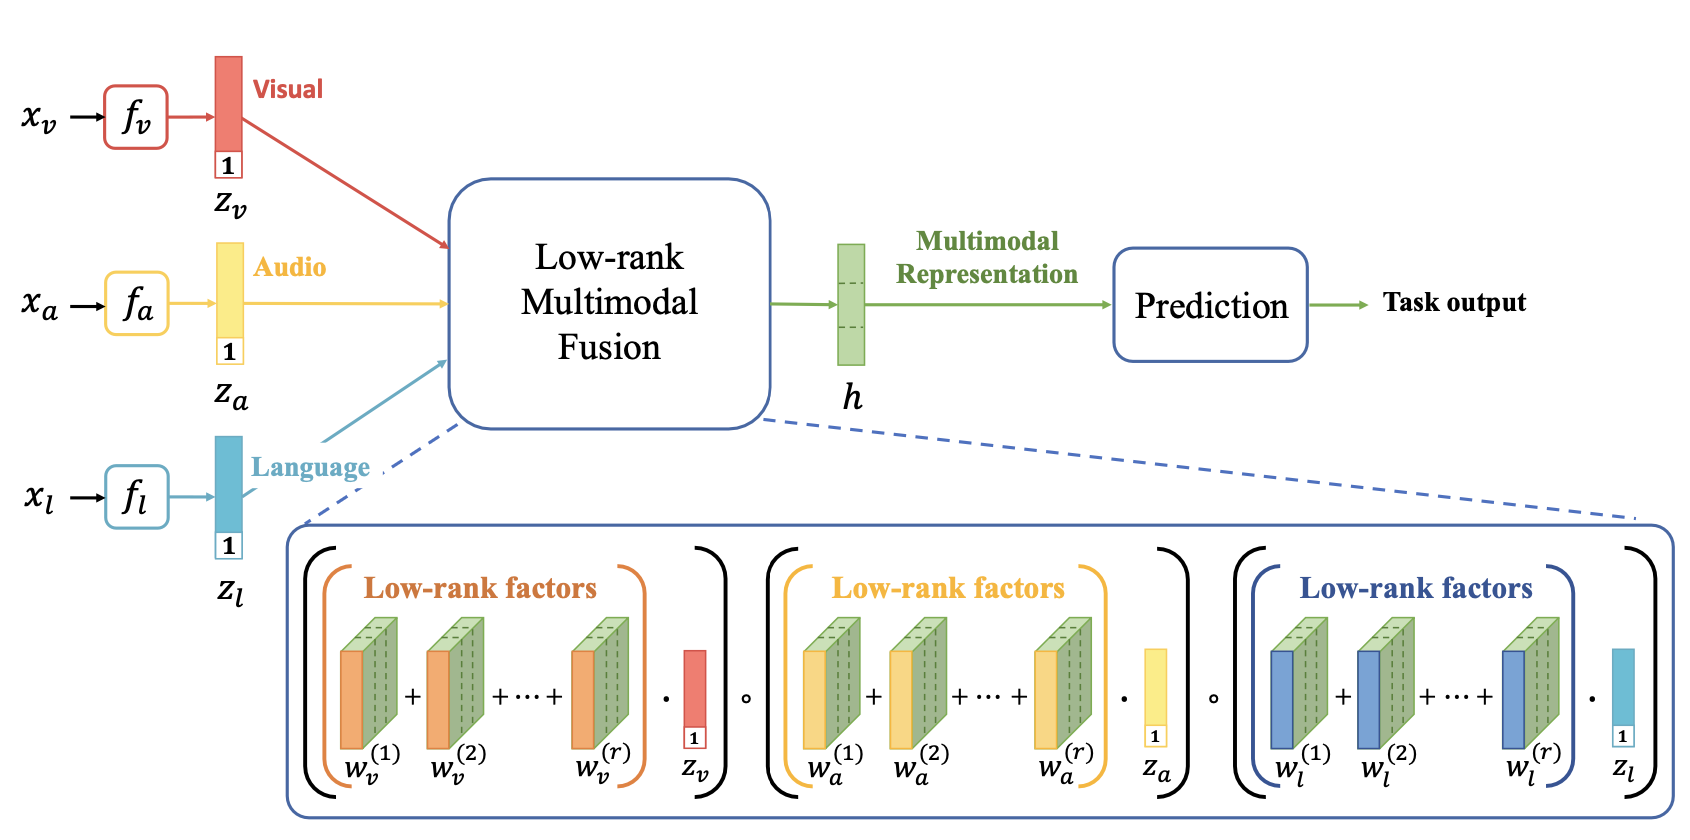
\includegraphics[width=1\linewidth]{Foundation model draft1//figs/LRTF.png}
    \caption{Overview of Low-rank Multimodal Fusion model structure: LMF first obtains the unimodal representation $z_a, z_v, z_l$ by passing the unimodal inputs $x_a, x_v, x_l$ into three sub-embedding networks $f_v, f_a, f_l$ respectively. LMF produces the multimodal output representation by performing low-rank multimodal fusion with modality-specific factors. The multimodal representation can be then used for prediction tasks. \cite{Liu2018EfficientLM} }
    
    \label{fig:LRTF}
\end{figure}

Beyond these fusion strategies, we also reimplemented several state-of-the-art multimodal models. Among them, Multimodal Transformer (MMT) achieved the best performance on CMU-MOSI, reinforcing the idea that Transformer-based multimodal interaction modeling is highly effective for emotion recognition tasks. However, its generalization ability slightly decreased on the more complex CMU-MOSEI dataset, despite still achieving strong performance. 

In contrast, Multimodal Factorization performed the worst, with an accuracy 10\%-15\% lower than other models, indicating that it might fail to effectively leverage multimodal information in emotion recognition tasks. We hypothesize that Multimodal Factorization may be more suitable for simpler multimodal tasks but struggles with complex affective computing problems, where interactions across modalities play a crucial role. Another interesting case is the Multimodal Cyclic Translation Network, which attempts to map information across different modalities, enabling one modality to be reconstructed from another. This approach performed well on CMU-MOSI (72.44\%) but significantly underperformed on CMU-MOSEI (59.49\%). This suggests that the cyclic translation approach does not generalize well to larger, more diverse datasets, as it may introduce noise or inconsistencies during cross-modal translation, leading to performance degradation on large-scale multimodal emotion recognition tasks.

\subsection{Inference Efficiency}
We observe that while Early Fusion and Late Fusion achieve strong performance, their high parameter count and computational cost make them less efficient. Furthermore, Early Fusion with GRU as the encoder leads to significantly poor performance, making it an impractical choice. In contrast, Late Fusion with GRU emerges as an optimal solution, as it offers a balance between efficiency and performance, making it a highly effective alternative.

Compared to Tensor Fusion, which computes the outer product between modalities, its computational requirements grow exponentially, making inference extremely expensive. Low-Rank Tensor Fusion (LRTF) effectively addresses this issue by applying low-rank factorization, significantly reducing the computational burden while maintaining performance comparable to full Tensor Fusion. Also, LRTF architecture requires fewer parameters compared to Tensor Fusion while maintaining the same level of accuracy.

\newpage
Despite Multimodal Cyclic Translation Network (MCTN) having a very small parameter size, its reliance on cyclic translation introduces additional forward passes, substantially increasing computational cost. As a result, despite its compact architecture, MCTN remains inefficient for inference.

Multimodal Transformer, on the other hand, suffers from O(N²) complexity due to the Self-Attention mechanism, causing inference cost to escalate rapidly with input length. Additionally, its high parameter count further contributes to computational inefficiency, making it less suitable for real-time applications.

Conversely, Multimodal Factorization, which is primarily based on low-rank decomposition, provides an extremely efficient solution by reducing the dimensionality of multimodal representations while preserving essential information. However, despite its efficiency, its performance in multimodal emotion recognition tasks remains suboptimal, indicating that factorization-based approaches may struggle to capture the intricate dependencies necessary for affective computing.

From an efficiency-driven perspective, Late Fusion with GRU provides the best trade-off between performance and computational cost, making it a practical and scalable solution. Meanwhile, LRTF emerges as an optimal alternative to Tensor Fusion, maintaining comparable accuracy while significantly reducing inference cost. In contrast, models such as MCTN and Multimodal Transformer suffer from high computational overhead due to cyclic translation and self-attention complexity, respectively. Finally, while Multimodal Factorization is the most computationally efficient model, its performance limitations suggest that efficiency alone is insufficient for robust multimodal emotion recognition, and a more nuanced balance between efficiency and multimodal representation learning is required.

\section{Future Works}

Based on the findings of this study, future work should focus on expanding experimental analysis, conducting ablation studies, and integrating large-scale pretrained multimodal models to further enhance the computational efficiency, recognition accuracy, and generalization capability of multimodal emotion recognition.

Our current experiments provide valuable insights into the performance and inference efficiency of different multimodal fusion strategies. However, to gain a deeper understanding of multimodal emotion recognition, further exploration is needed. Future research should investigate additional fusion architectures, such as Graph Neural Networks (GNNs) and Diffusion Models, to enhance the modeling of multimodal interactions. Additionally, evaluating model generalization across diverse datasets remains an open challenge. Expanding experiments to broader datasets such as MELD  \cite{poria2019meld} would enable a more comprehensive assessment of the applicability of different fusion strategies in varying contexts, ultimately improving model adaptability across different scenarios.

A systematic ablation study is also essential to quantify the contributions of different modalities and their combinations to overall model performance. This includes evaluating the effectiveness of unimodal (text, audio, or visual) inputs, as well as various modality combinations (e.g., text + audio, text + visual) to determine their respective impacts. Furthermore, future research should explore adaptive modality weighting mechanisms, allowing models to dynamically adjust modality contributions based on specific emotion categories. This would address the limitations of fixed fusion strategies and enhance model flexibility.

For pretrained multimodal models such as CLIP, GPT-4, and Flamingo, future research should also explore how to effectively leverage these powerful pretrained models to improve multimodal emotion recognition while optimizing inference efficiency. Specifically, pretrained visual models (e.g., CLIP) could be utilized for visual feature extraction, while large-scale language models (e.g., LLaMA, T5) could enhance text-based emotion recognition, enabling a more robust and comprehensive multimodal understanding. Given the substantial computational cost associated with large models, future work should also investigate parameter-efficient fine-tuning (PEFT) techniques, such as LoRA and Adapter-Tuning, to adapt these models to multimodal emotion analysis with lower computational overhead.

\section{Limitions}
Despite the promising results obtained from our multimodal emotion recognition study, several limitations should be acknowledged. First, our experiments were conducted on two datasets—CMU-MOSI and CMU-MOSEI—that differ significantly in scale. This discrepancy in dataset size may introduce biases in performance evaluation and limit the generalizability of our findings. Moreover, the number of datasets used for comparative analysis is relatively small, which restricts our ability to draw comprehensive conclusions about the relative suitability of the various architectures examined.

Another notable limitation is the insufficient exploration of emotion shift—a critical aspect of multimodal emotion recognition. Emotion shift refers to the dynamic transition of emotional states over time, which is particularly prevalent in natural conversational settings. Our current approach does not delve into the deeper causes or the modeling of these temporal variations, nor does it address the nuances of how changes in features—such as variations in speech waveforms—impact the recognition of evolving emotional expressions.

In future work, we plan to mitigate these limitations by incorporating additional conversational datasets, such as MELD, which are well-suited for examining emotion shift dynamics. This extension will allow us to focus on capturing and analyzing fine-grained changes in emotional expressions across modalities, thereby deepening our understanding of the phenomenon and informing further architectural improvements.


\bibliographystyle{alpha}
\bibliography{main}

\end{document}